\documentclass[a4paper, 11pt]{article}

\usepackage{comment} % enables the use of multi-line comments (\ifx \fi) 
\usepackage{fullpage} % changes the margin
\usepackage{vhistory}
\usepackage{enumitem}
\usepackage{graphicx}

\newlength{\drop}

\newcommand\tab[1][1cm]{\hspace*{#1}}

\begin{document}
    
    
    \begin{titlepage}
        \drop=0.1\textheight
        \centering
        \vspace*{\baselineskip}
        \rule{\textwidth}{1.6pt}\vspace*{-\baselineskip}\vspace*{2pt}
        \rule{\textwidth}{0.4pt}\\[\baselineskip]
        {\LARGE \textbf{USER HANDBOOK \\ PROJECT 1 : ADDRESS BOOK}}\\[0.2\baselineskip]
        \rule{\textwidth}{0.4pt}\vspace*{-\baselineskip}\vspace{3.2pt}
        \rule{\textwidth}{1.6pt}\\[\baselineskip]
        \scshape
        \vspace*{2\baselineskip}
        Edited by \\[\baselineskip]
        {\Large Frazer Bayley \\ Haley Whitman \\ Abdulaziz Al-Heidous \\ Alison Legge \\ Jeremy Brennan\par}

        \vfill
        {\scshape \LARGE Project 1 -} \        {\LARGE Team 3}\par
    \end{titlepage}


\tableofcontents
\vspace*{25\baselineskip}
\begin{versionhistory}
    \vhEntry{.1}{26.01.17}{Frazer Bayley}{Created the first draft of the document, 1 - 9}
    \vhEntry{.2}{28.01.17}{Frazer Bayley}{Adding more of the functionality, 10 - 15}
    \vhEntry{.3}{30.01.17}{Frazer Bayley}{Adding Screenshots}
\end{versionhistory}
\pagebreak


\section{Introduction}
\subsection{A Simple Address Book}
Thank you for using this simple Address Book. This Address Book is designed for an average person who may have tens to hundreds of contacts. It provides functionality that you would expect to have in a simple Address Book, such as adding contacts, editing or deleting a contact, etc. 
\subsection{How to Use this Handbook}
This handbook covers a range of scenarios you might encounter when using this Address Book. This handbook will walk you through each scenario step by step.
\begin{itemize}
    \item \textbf{Read Every Step:} \\ Make sure you do not skip any steps that are listed in this handbook. Every step has been carefully thought out to make using the Address Book easier.
    \item \textbf{Use the Handbook in Conjunction with the Address Book:} \\ After your first read through of the handbook have it open and ready as you first start to use the Address Book.
    \item \textbf{Experiencing Issues:} \\ If you are experiencing further issues and are unable to solve it with the help of this handbook, please contact our support team.
\end{itemize}

\clearpage

\section{Getting Started with the Address Book}
\subsection{Download and Install}
\subsection{Starting the Application}

\clearpage

\section{Adding Contacts}
\subsection{Overview}
Adding a new contact is easy to do in this Address Book. It will only take a few clicks.
\subsection{Procedure}
\begin{enumerate}[label=\textbf{\arabic*})]
    \item{\textbf{Begin at the Main Page}}\\ Begin at the main page of the Address Book. Below are two images of the main page to help you verify you are where you need to be.
    
    \begin{figure}[h!]
    \centering
      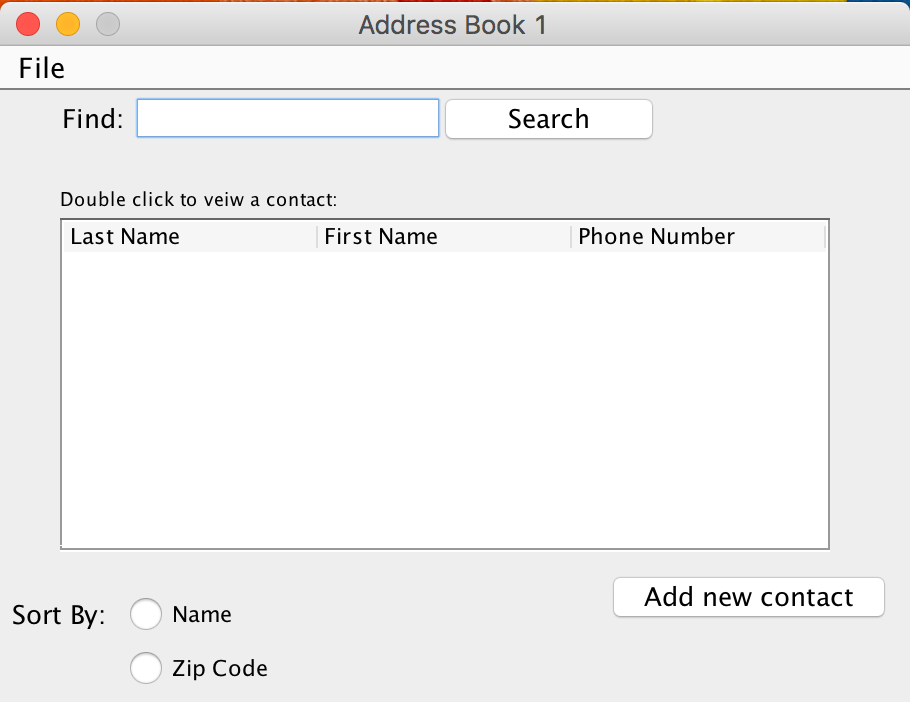
\includegraphics[width=250]{main_page_empty.png}
      \caption{Empty Main Page}
    \end{figure}

    \begin{figure}[h!]
    \centering
      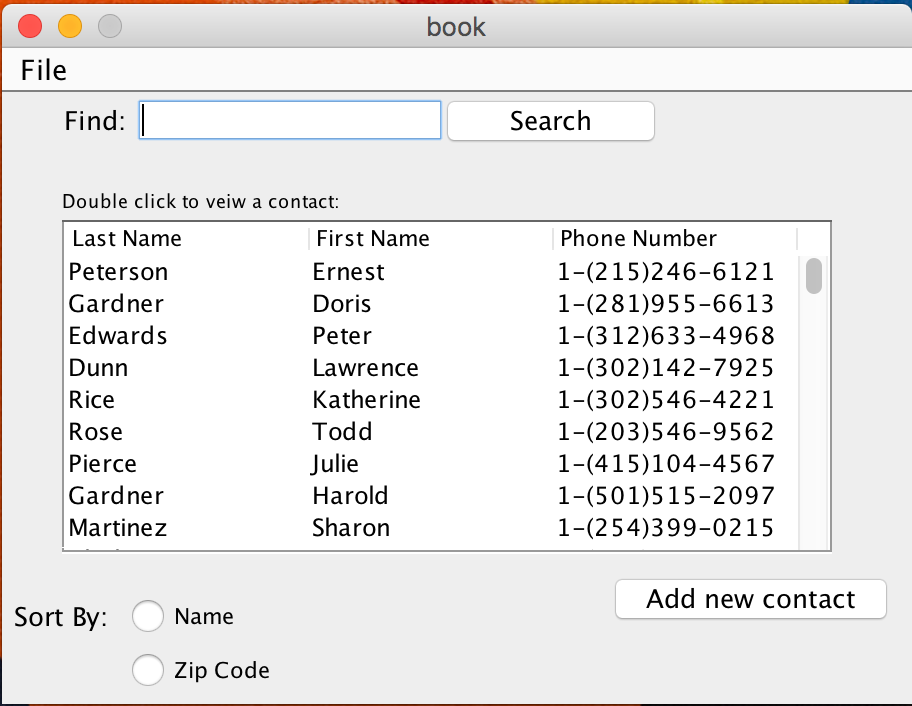
\includegraphics[width=250]{main_page_full.png}
      \caption{Full Main Page}
    \end{figure}
    
    \clearpage

    \item{\textbf{Click the "Add Contact" Button}}\\ You will see an "Add Contact" button on the main window. Move the mouse to it and click the "Add Contact" button. Upon clicking the Add Contact window will appear.
    
    \begin{figure}[h!]
    \centering
      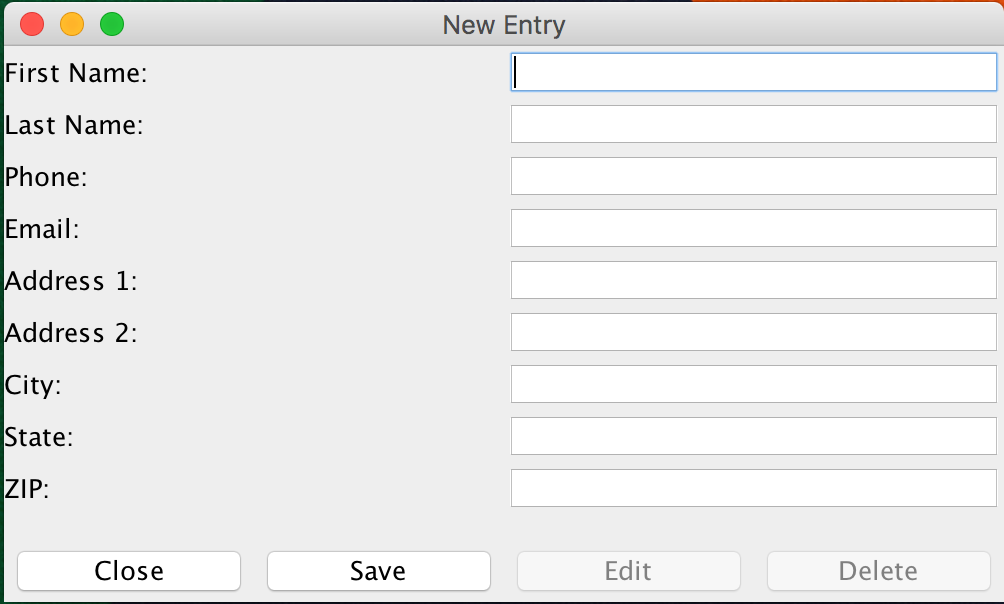
\includegraphics[width=250]{add_new_contact_window.png}
      \caption{Add Contact Window}
    \end{figure}
    
    \item{\textbf{Fill In Contact Data}}\\ The Add Contact window has multiple fields for you to fill in with Contact information. You are required to enter a first name or a last name, plus a second entry of the ones laid out.
    
    \begin{figure}[h!]
    \centering
      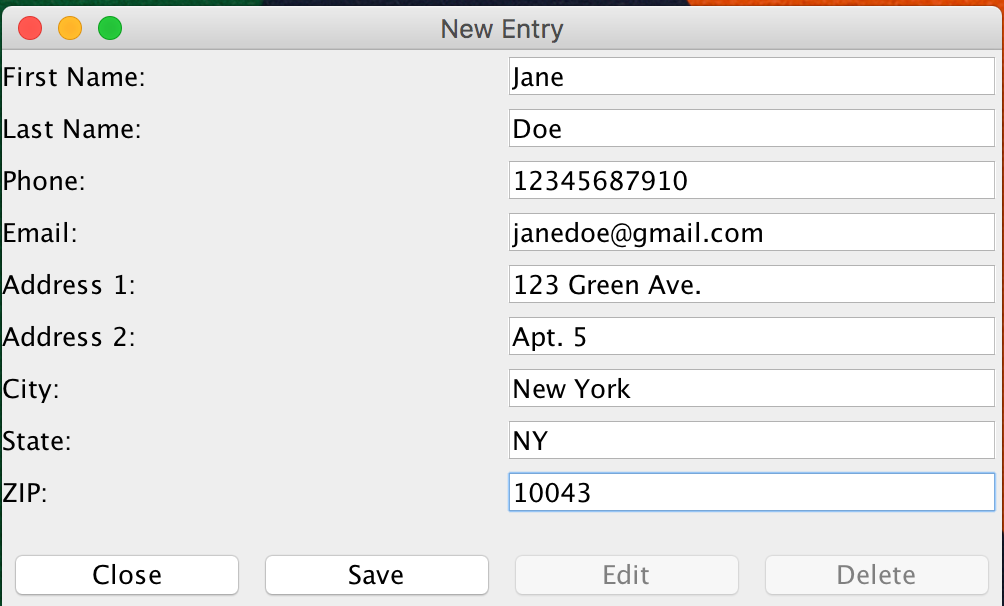
\includegraphics[width=250]{new_contact_entry.png}
      \caption{Contact Entries}
    \end{figure}
    
    \clearpage
    
    \item{\textbf{Save New Contact Information}}\\ When you have entered all the information you wish to enter about your new contact click the "Save" button. This will permanently save the Contact to the Address Book. If you haven't entered all the required information detailed in the last step an error message will appear directing you back to the Add Contact window. It will keep doing this until the information is entered correctly.
    
    \begin{figure}[h!]
    \centering
      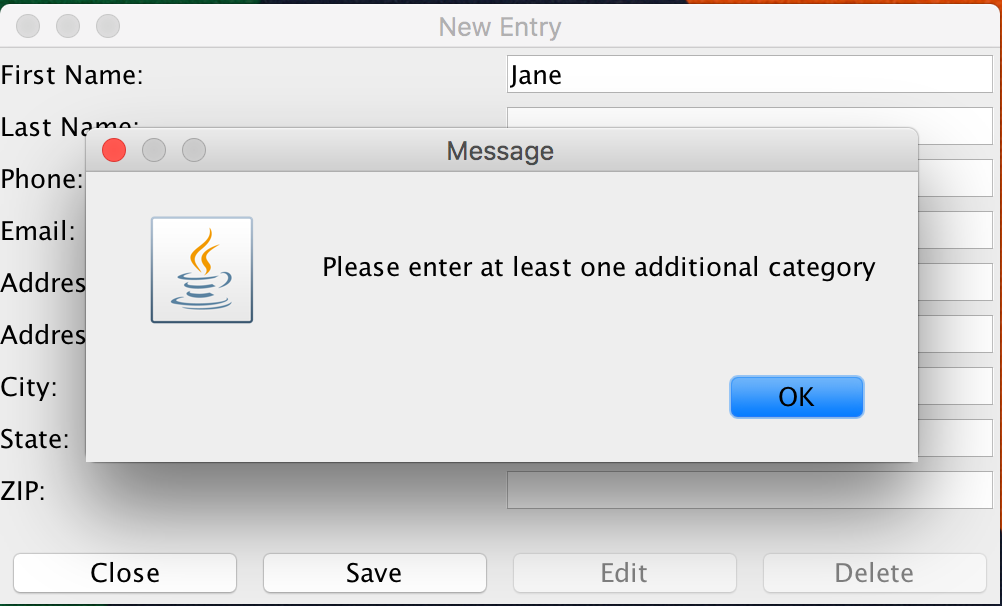
\includegraphics[width=250]{add_entry_error.png}
      \caption{Not Enough Entries}
    \end{figure}
    
    \item{\textbf{Close Add Contact Window}}\\ Now that you have saved the Contact information, click the "Close" button. This will close and remove the Add Contact window from the screen. If you have not saved the information before this step a dialogue box will appear asking you if you would like to Save the new information or Discard the new information.
    
    \begin{figure}[h!]
    \centering
      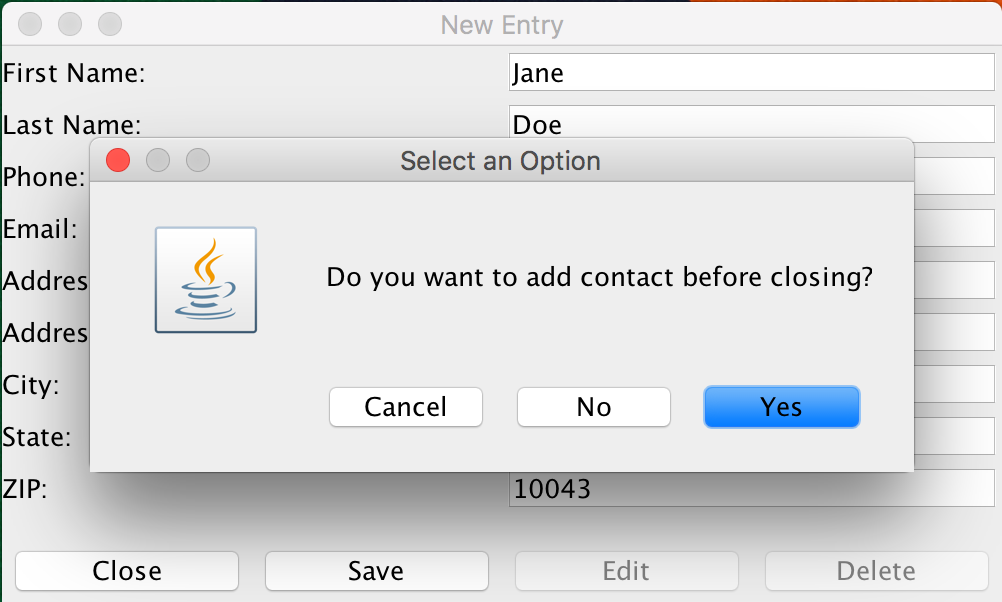
\includegraphics[width=250]{add_entry_save_error.png}
      \caption{Prompt to Save}
    \end{figure}
    
    \clearpage
    
    After this step you will be left with the Main page of the Address Book. If you scroll through the entries you will see your newly added Contact listed.
    
    \begin{figure}[h!]
    \centering
      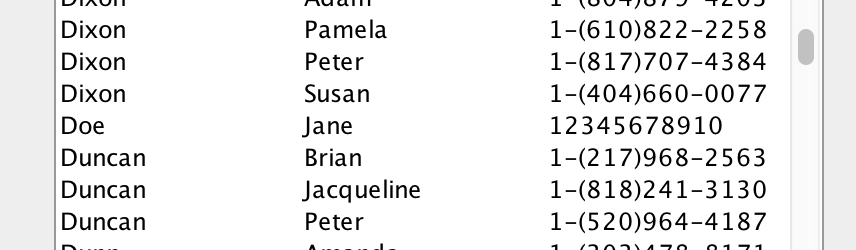
\includegraphics[width=250]{jane_doe_added.png}
      \caption{New Entry Added to Address Book}
    \end{figure}
   
\end{enumerate}

\clearpage

\section{Selecting Contacts}
\subsection{Overview}
You will eventually need to look at the information of a Contact in your Address Book. Here is how to do so.
\subsection{Procedure}
\begin{enumerate}[label=\textbf{\arabic*})]
    \item{\textbf{Begin at the Main Page of a Non Empty Address Book}}\\ To use this feature you must have at least one Contact in your address book.
    
    \begin{figure}[h!]
    \centering
      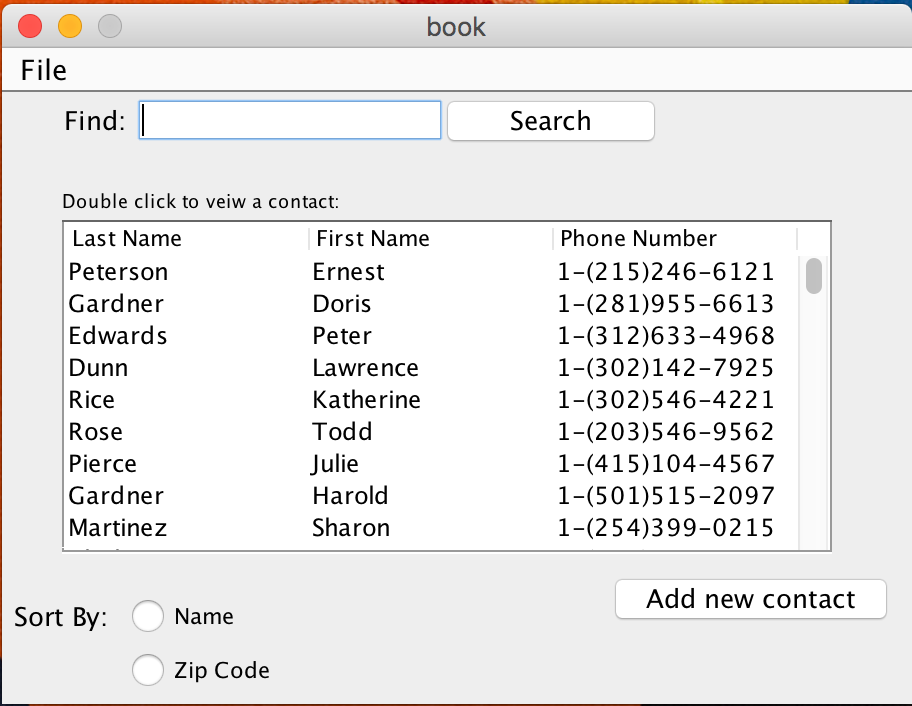
\includegraphics[width=250]{main_page_full.png}
      \caption{Full Main Page}
    \end{figure}
    
    \item{\textbf{Find Contact For Selection}}\\ Find the contact you would like to Select by scrolling through the list of Contacts. Hover your mouse over the desired Contact. 
    
    \begin{figure}[h!]
    \centering
      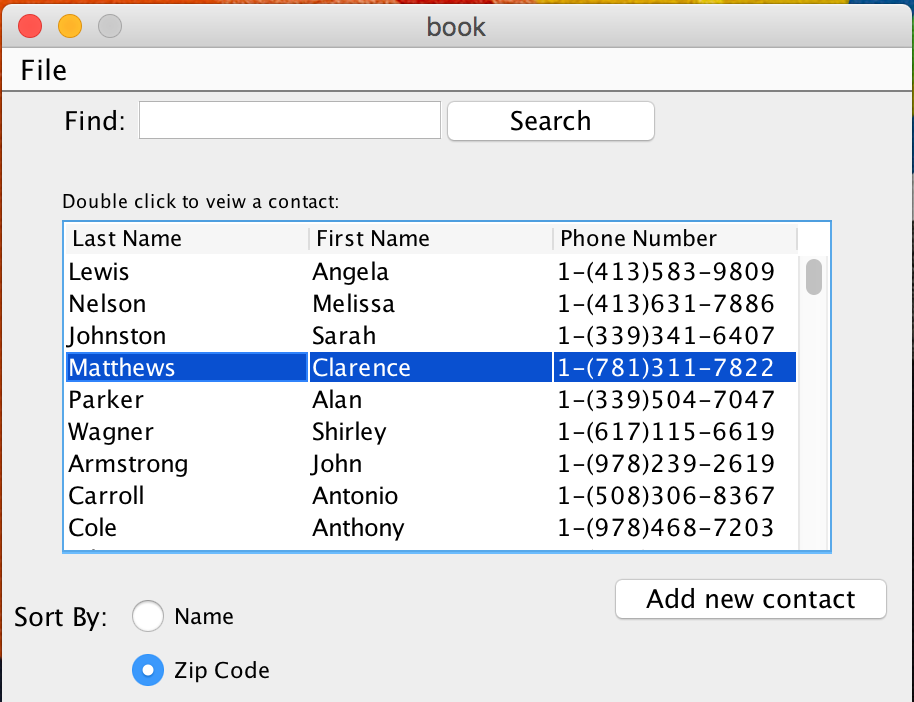
\includegraphics[width=250]{main_screen_select.png}
      \caption{Selecting a Contact}
    \end{figure}
    
    \item{\textbf{Double Click Contact}}\\ With the mouse over the desired Contact, double click the Contact. This will make the Contact information appear in another window.
    
    \begin{figure}[h!]
    \centering
      \includegraphics[width=250]{select_contact.png}
      \caption{Viewing Contact}
    \end{figure}
    
    \item{\textbf{Close Window}}\\ Once you are done with viewing the contact information, click the "Close" button. This will remove the Contact window from view.

\end{enumerate}

\clearpage

\section{Editing Contacts}
\subsection{Overview}
If you wish to make changes to an existing contact the steps below detail how to do so.
\subsection{Procedure}
\begin{enumerate}[label=\textbf{\arabic*})]
    \item{\textbf{Select Contact for Editing}}\\ Complete steps 1, 2, and 3 of the "Selecting Contacts" section of this handbook. 
    
    \item{\textbf{Click the "Edit" Button}}\\ You should be looking at the Contact information page. Click the "Edit" button.
    
    \item{\textbf{Edit Information}}\\ This will make it so the the information in the field boxes are editable. Change or add any information you desire. 
    
    \begin{figure}[h!]
    \centering
      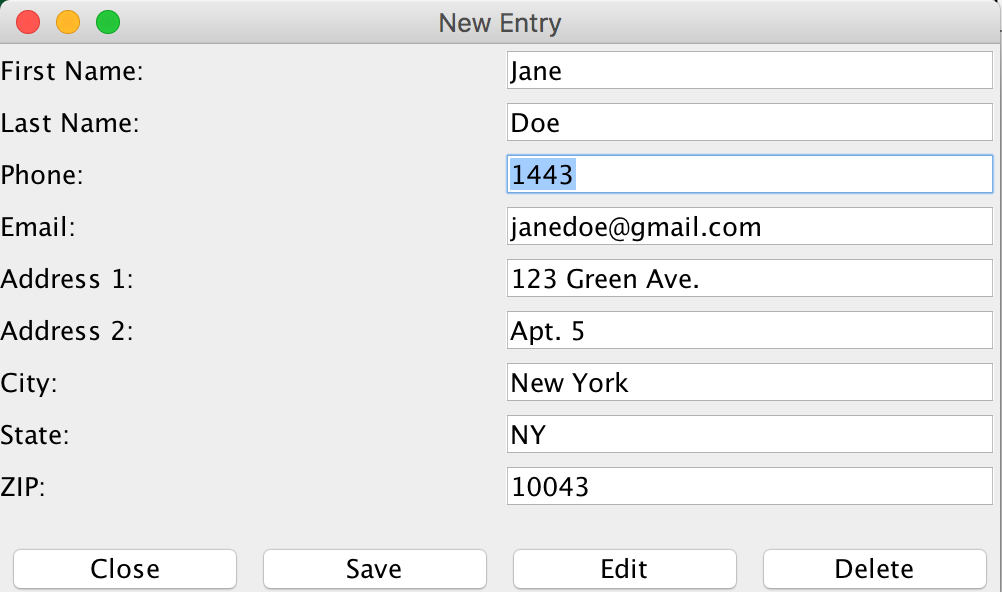
\includegraphics[width=250]{edit_contact.png}
      \caption{Editing a Contact}
    \end{figure}
    
    \item{\textbf{Save Newly Edited Information}}\\ Click the "Save" button to permanently save the changes you have made to the Contact.
    
    \clearpage
    
    \item{\textbf{Close Window}}\\ Once you are done with saving the contact information, click the "Close" button. This will remove the Contact window from view. If you haven't clicked the "Save" button before this step a dialog box will appear asking you if you want to Save the changes you have made or Discard them.
    
    \begin{figure}[h!]
    \centering
      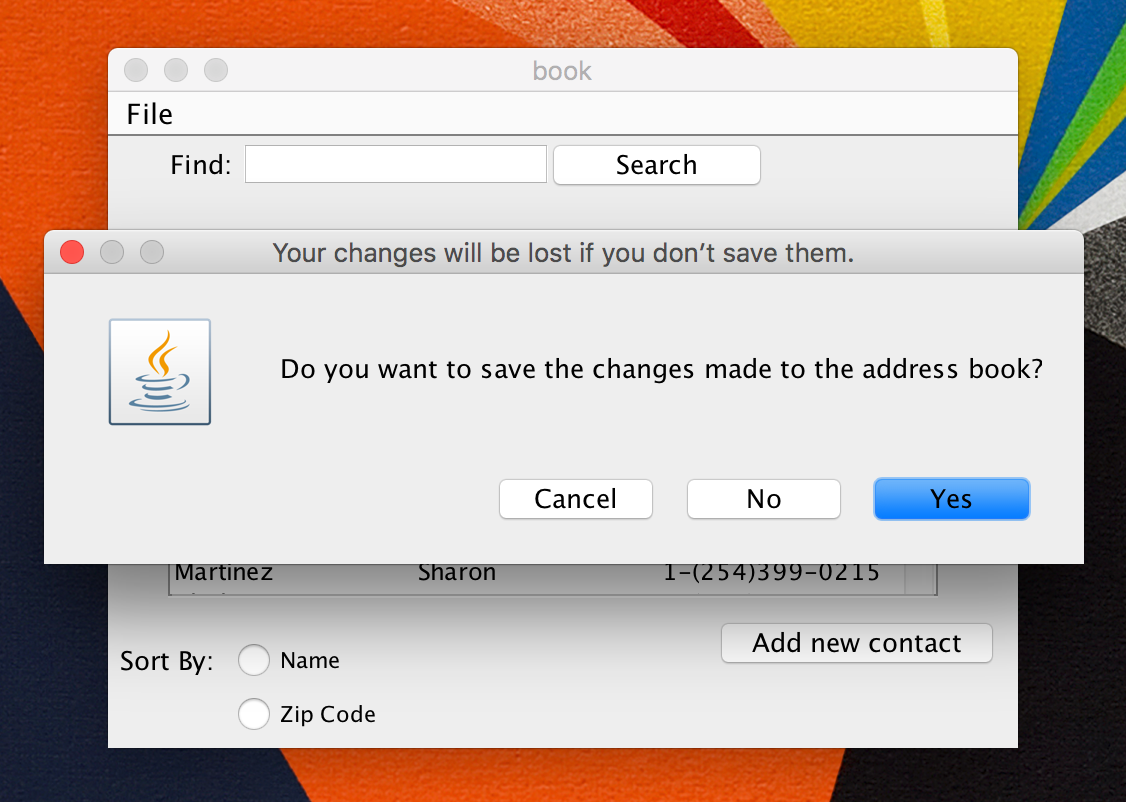
\includegraphics[width=250]{close_save_error.png}
      \caption{Prompt to Save}
    \end{figure}
\end{enumerate}

\clearpage

\section{Deleting Contacts}
\subsection{Overview}
If you wish to remove a Contact completely from your Address Book follow the steps below.
\subsection{Procedure}
\begin{enumerate}[label=\textbf{\arabic*})]
    \item{\textbf{Select Contact for Editing}}\\ Complete steps 1, 2, and 3 of the "Selecting Contacts" section of this handbook. 
    
    \item{\textbf{Click the "Delete" Button}}\\ You should be looking at the Contact information page. Click the "Delete" button. Once you have clicked the Delete button a dialogue box should appear asking if you are sure about your decision to delete. If you are sure click "Yes", if not click "No".
    
    Image dialogue box
    
    After you select "Yes" the Contact information window will disappear from view. If you selected "No" you will have to follow the normal procedure of closing the window detailed in previous sections to remove the Contact Information from view.  
\end{enumerate}

\clearpage

\section{Sort Address Book}
\subsection{Overview}
If you want to see the list of contacts in either Descending by last name or Ascending by zip code then follow these steps. 
\subsection{Procedure}
\begin{enumerate}[label=\textbf{\arabic*})]
    \item{\textbf{Begin at the Main Page of Non Empty Address Book}}\\ For this feature to work your Address Book must contain at least two Contacts.
    
    \begin{figure}[h!]
    \centering
      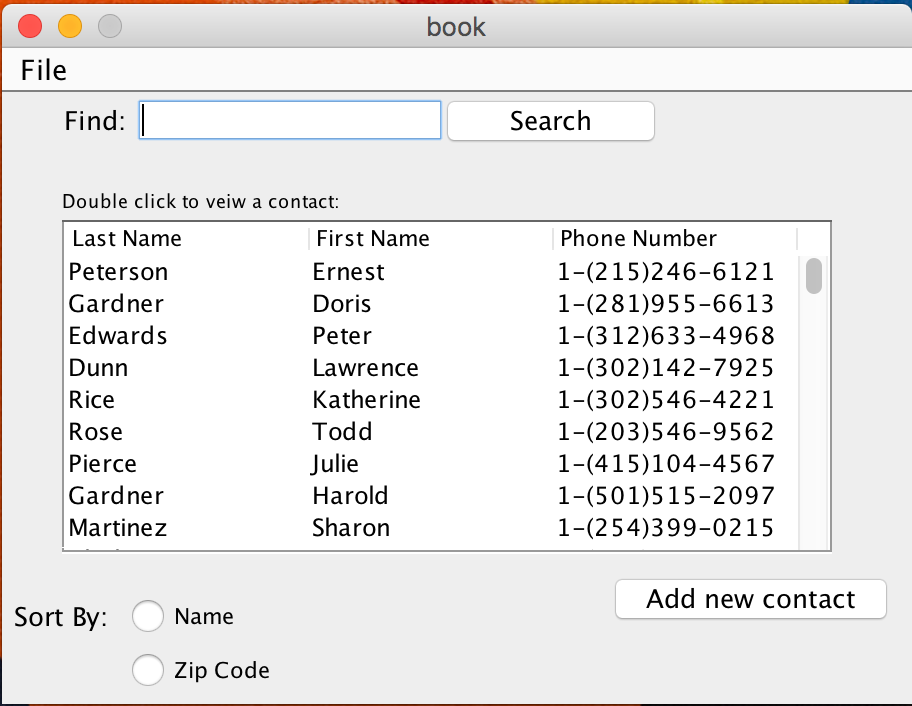
\includegraphics[width=250]{main_page_full.png}
      \caption{Full Main Page}
    \end{figure}
    
    \item{\textbf{Order by Last Name}}\\ Click the button that says "Order by Last Name". Once selected you will see the ordering change as long as it wasn't in that order before. 
    
    \item{\textbf{Order by Zip Code}}\\ Click the button that says "Order by Zip Code". Once selected you will see the ordering change as long as it wasn't in that order before.
\end{enumerate}

\clearpage

\section{Search}
\subsection{Overview}
If you would like to find a specific Contact without scrolling through the list of them follow the procedure below.
\subsection{Procedure}
\begin{enumerate}[label=\textbf{\arabic*})]
    \item{\textbf{Begin at the Main Page of Non Empty Address Book}}\\ For this feature to work your Address Book must contain at least two Contacts.
    
    \begin{figure}[h!]
    \centering
      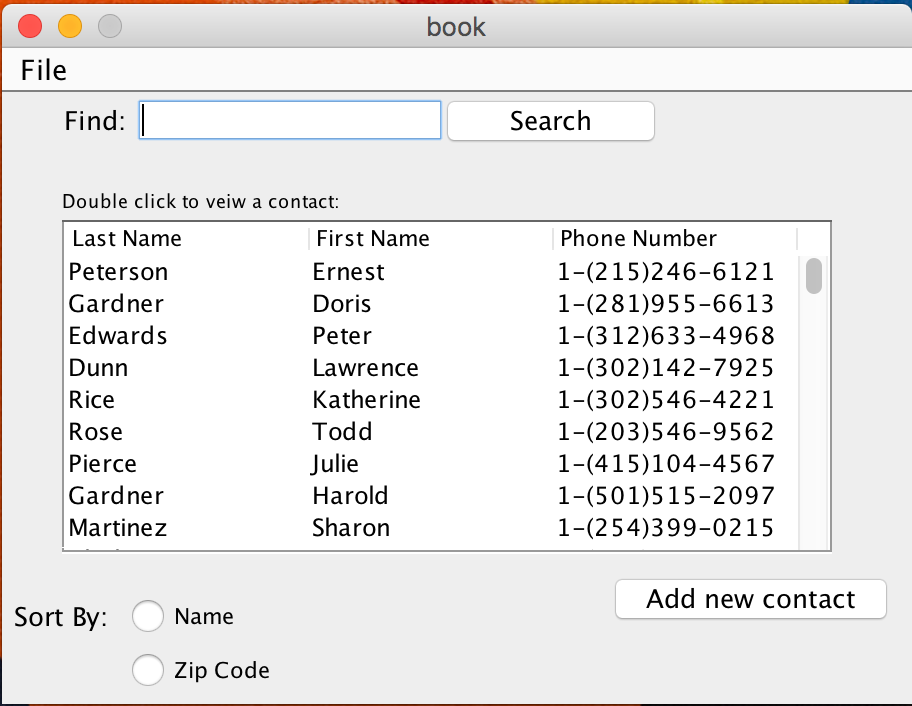
\includegraphics[width=250]{main_page_full.png}
      \caption{Full Main Page}
    \end{figure}
    
    \item{\textbf{Find the Search Bar}}\\ On the page there will be a field where you can make entries. 
    
    \begin{figure}[h!]
    \centering
      \includegraphics[width=250]{search_bar.png}
      \caption{Search Bar}
    \end{figure}
    
    \clearpage
    
    \item{\textbf{Enter Your Search}}\\ In the text entry field enter anything related to the Contact you wish to view. Once you type your query, click "Search". If there are any contacts matching your query they will present themselves in the scroll box.
    
    \begin{figure}[h!]
    \centering
      \includegraphics[width=250]{search_results.png}
      \caption{Search Results}
    \end{figure} 
    
    \item{\textbf{Getting Out of Your Results}}\\ To go back to the main page with all your Contacts clear the Search bar of text and click "Search".

\end{enumerate}

\clearpage

\section{Create New Address Book}
\subsection{Overview}
When you first launch the Address Book application you will always open up to a "New" address book. If you would like to create a new address book when you have an existing address book already open follow this procedure. 
\subsection{Procedure}
\begin{enumerate}[label=\textbf{\arabic*})]
    \item{\textbf{Begin at the Main Page of the Address Book}}\\ Make sure you are at the Main page of the Address Book.
    
    \begin{figure}[h!]
    \centering
      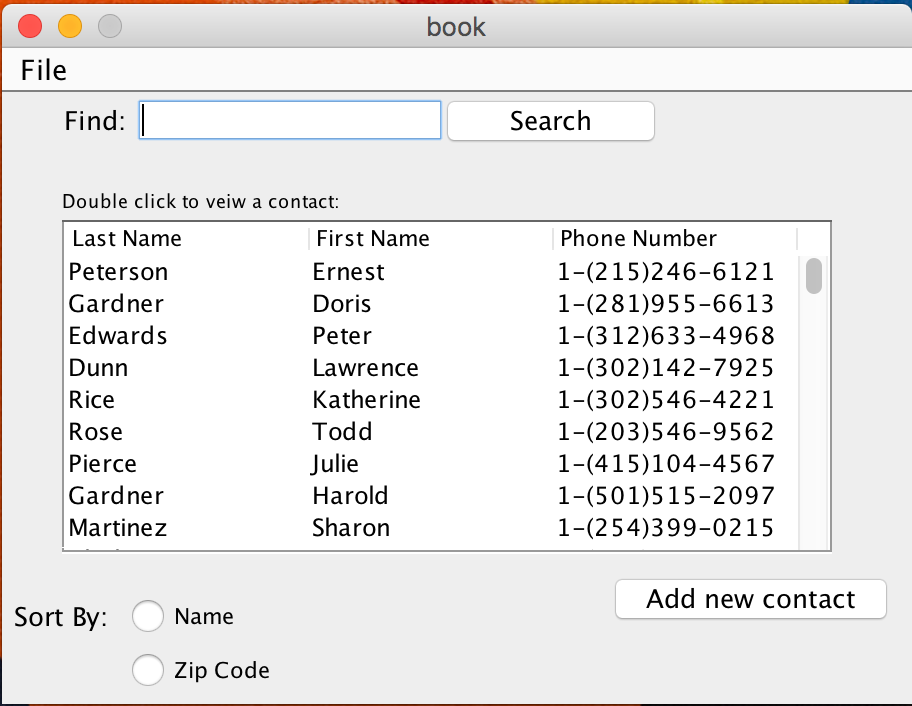
\includegraphics[width=250]{main_page_full.png}
      \caption{Full Main Page}
    \end{figure}
    
    \item{\textbf{Select the File Menu}}\\ At the top of the Main page window there will be a button that reads "File". Select it and a menu will pop open.
    
    \begin{figure}[h!]
    \centering
      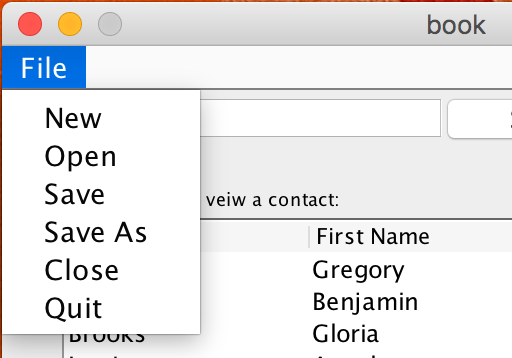
\includegraphics[width=250]{file_menu.png}
      \caption{File Menu}
    \end{figure} 
    
    \item{\textbf{Select "New"}}\\ Click the "New" option in the menu. This will create a blank Address Book in another window.
    
    \begin{figure}[h!]
    \centering
      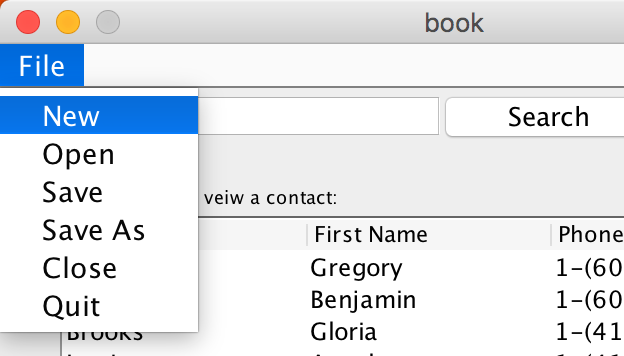
\includegraphics[width=250]{new_selection.png}
      \caption{Select New}
    \end{figure}
    
    \begin{figure}[h!]
    \centering
      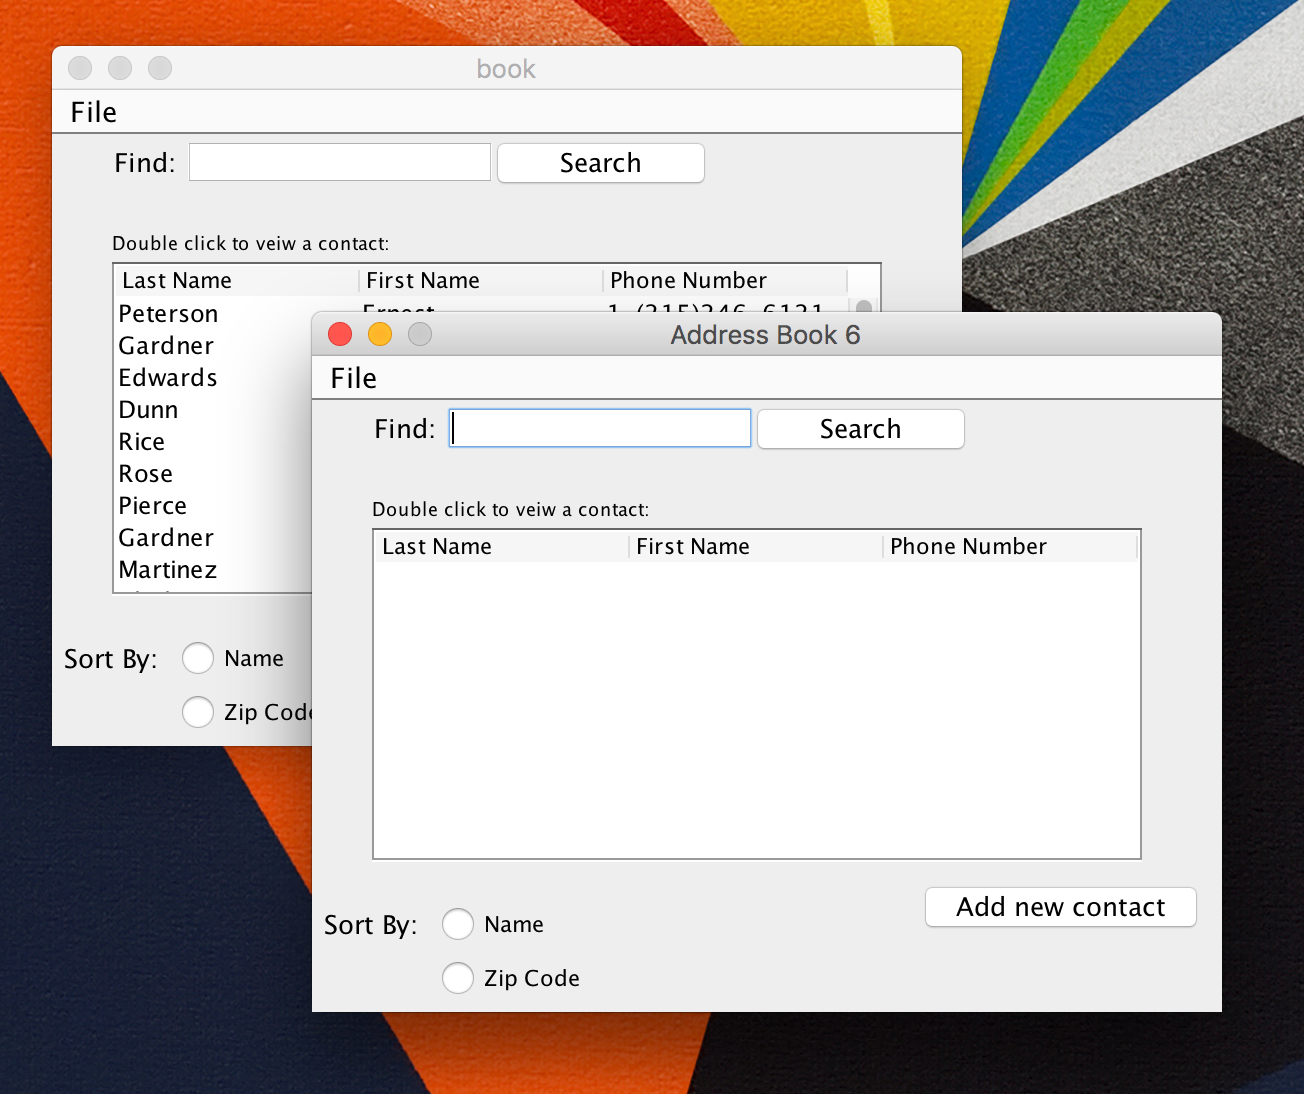
\includegraphics[width=250]{new_address_book.png}
      \caption{New Address Book}
    \end{figure}
    
    Now you can use your New Address Book.
\end{enumerate}

\clearpage

\section{Save Address Book to File}
\subsection{Overview}
At some point you will want to save the entire Address Book. The procedure below walks you through how to do so.
\subsection{Procedure}
\begin{enumerate}[label=\textbf{\arabic*})]
    \item{\textbf{Begin at the Main Page of the Address Book}}\\ Make sure you are at the Main page of the Address Book.
    
    \begin{figure}[h!]
    \centering
      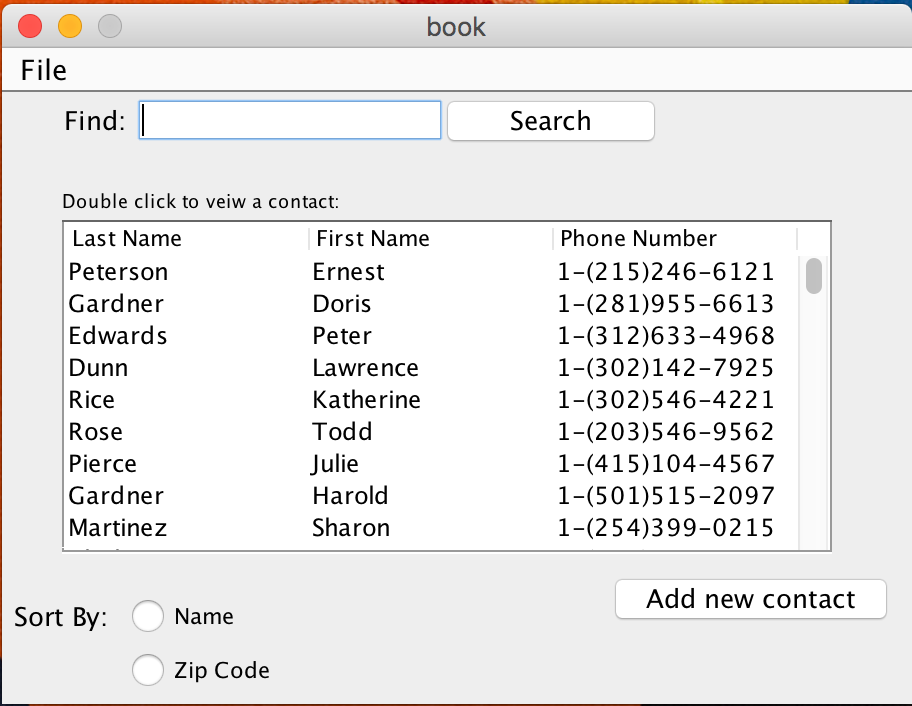
\includegraphics[width=250]{main_page_full.png}
      \caption{Full Main Page}
    \end{figure}
    
    \item{\textbf{Select the File Menu}}\\ At the top of the Main page window there will be a button that reads "File". Select it and a menu will pop open.
    
    \begin{figure}[h!]
    \centering
      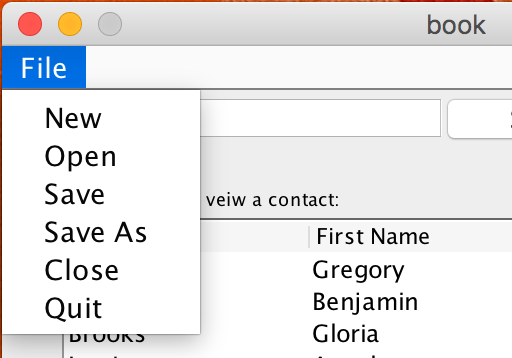
\includegraphics[width=250]{file_menu.png}
      \caption{File Menu}
    \end{figure}  
    
    \clearpage
    
    \item{\textbf{Select "Save"}}\\ Click the "Save" option in the File menu. This feature will Save the Address Book to a predetermined file, the file you opened the Address Book from. After you have clicked "Save" the Address Book and its entire contents will be safely stored. 
    
    \begin{figure}[h!]
    \centering
      \includegraphics[width=250]{save_selection.png}
      \caption{Select Save}
    \end{figure}
\end{enumerate}

\clearpage

\section{Save As and Renaming Your Address Book}
\subsection{Overview}
If you would like to Save your Address Book under a different name and/or in a different location follow the below procedure to do so.
\subsection{Procedure}
\begin{enumerate}[label=\textbf{\arabic*})]
    \item{\textbf{Begin at the Main Page of the Address Book}}\\ Make sure you are at the Main page of the Address Book.
    
    \begin{figure}[h!]
    \centering
      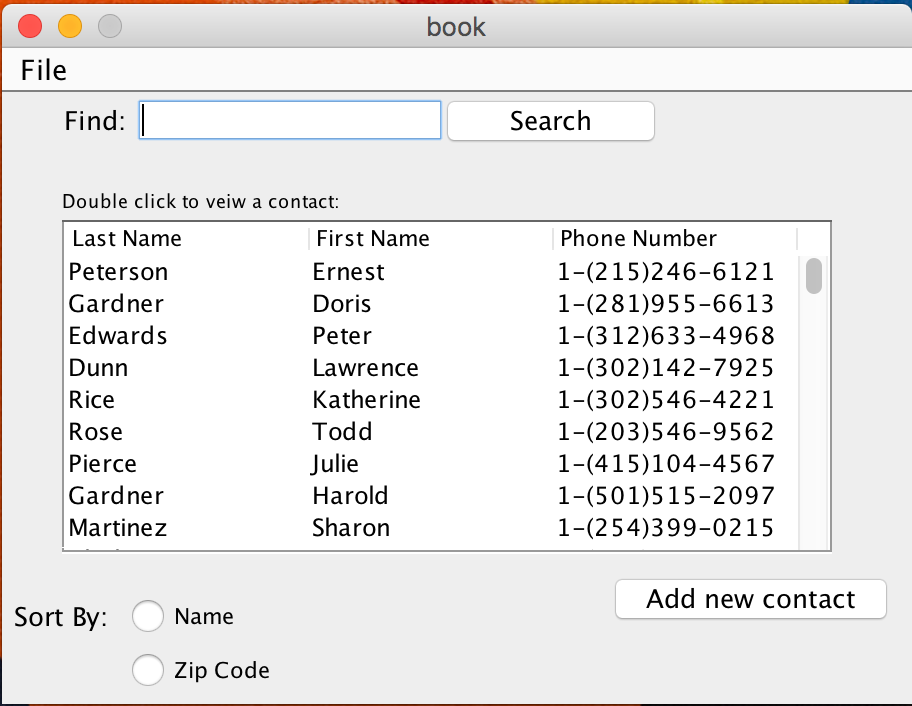
\includegraphics[width=250]{main_page_full.png}
      \caption{Full Main Page}
    \end{figure}
    
    \item{\textbf{Select the File Menu}}\\ At the top of the Main page window there will be a button that reads "File". Select it and a menu will pop open.
    
    \begin{figure}[h!]
    \centering
      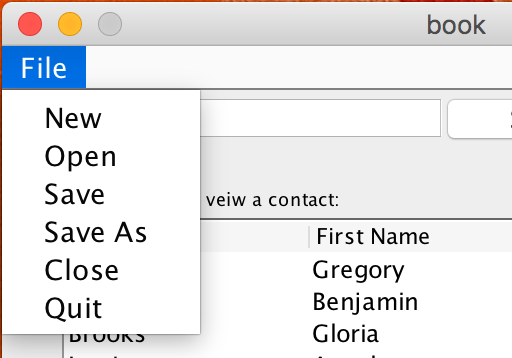
\includegraphics[width=250]{file_menu.png}
      \caption{File Menu}
    \end{figure}   
    
    \clearpage
    
    \item{\textbf{Select "Save As"}}\\ Click the "Save As" button and a pop up window will appear.
    
    \begin{figure}[h!]
    \centering
      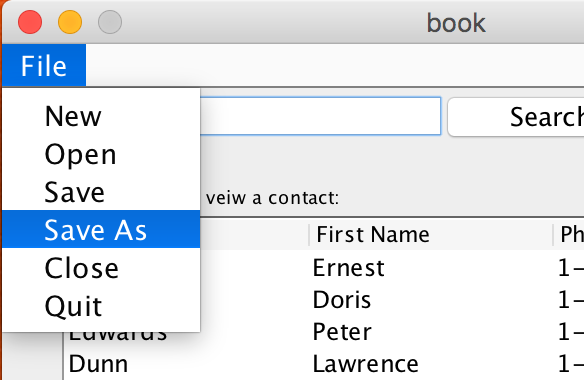
\includegraphics[width=250]{save_as_selection.png}
      \caption{Select Save As}
    \end{figure}
    
    \item{\textbf{Write in New File Name}}\\ In the new window you will be asked for a new file name and where to save the file. Make your choices and then hit "Save". After this step your Address Book will have a new name and file path.
    
    \begin{figure}[h!]
    \centering
      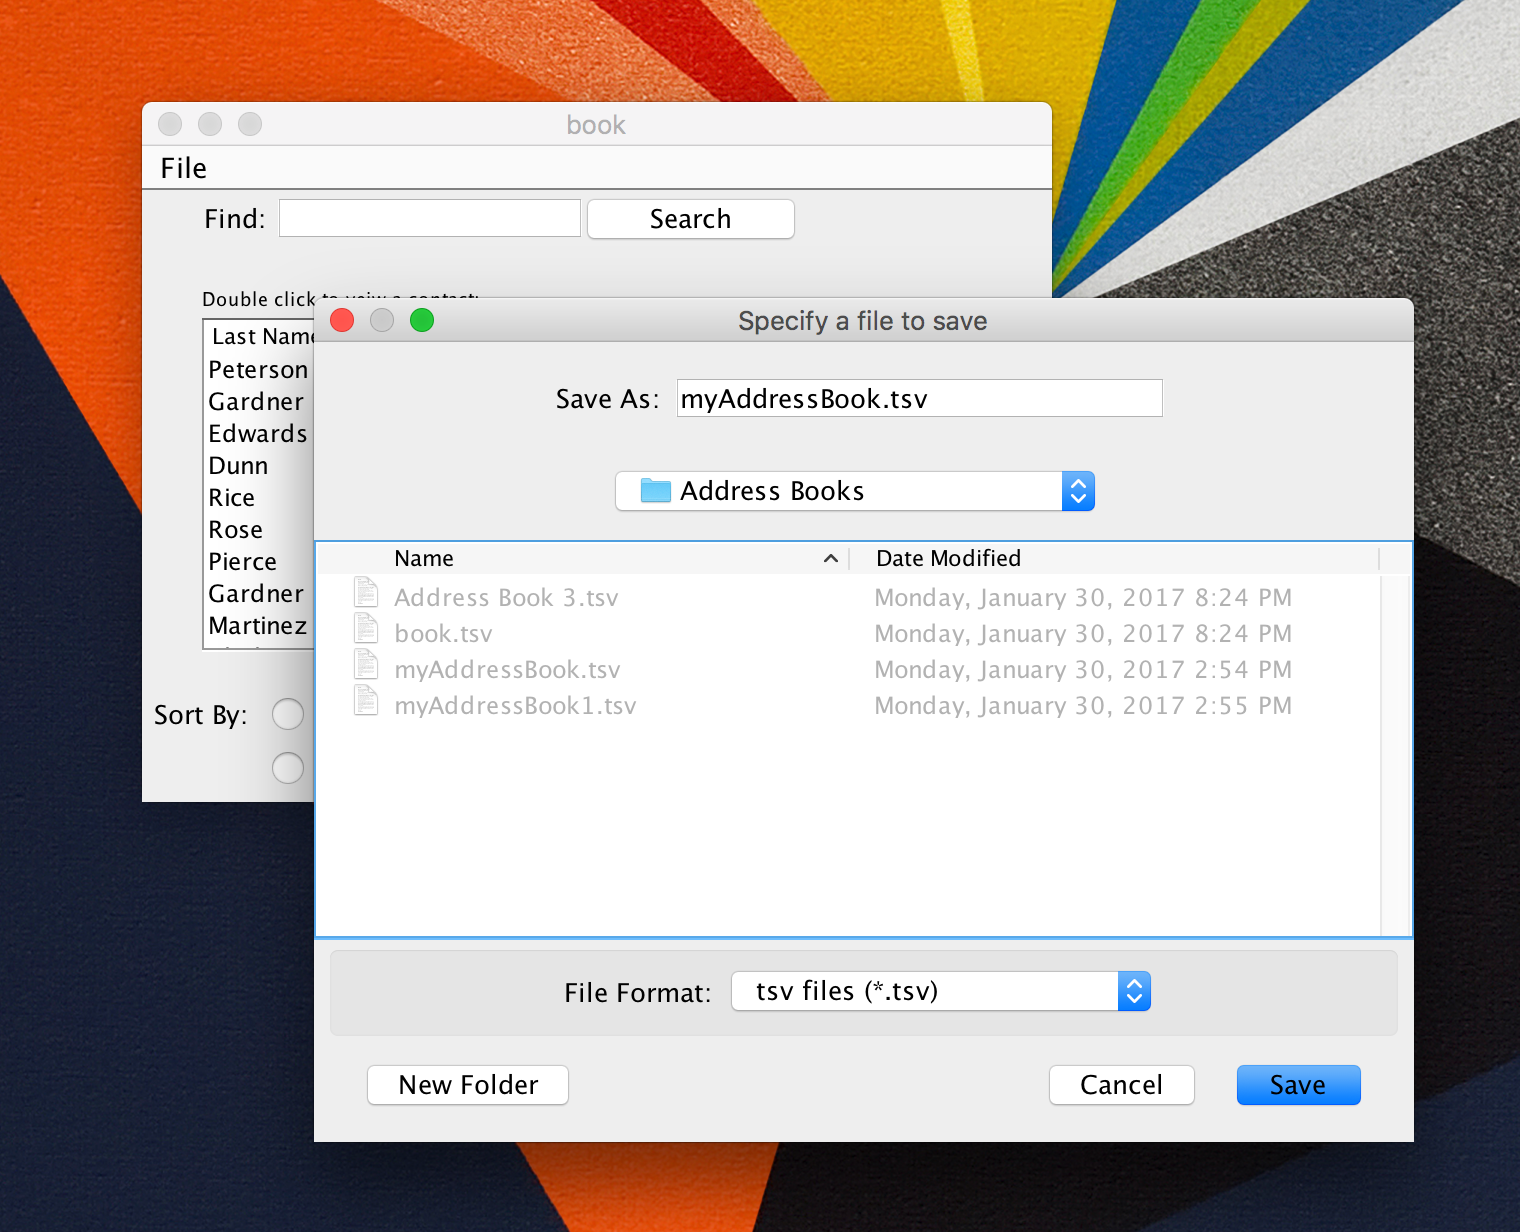
\includegraphics[width=250]{save_as_window.png}
      \caption{Save As Window}
    \end{figure}
\end{enumerate}

\clearpage

\section{Open Existing Address Book}
\subsection{Overview}
If you want to Open an existing Address Book follow the procedure below.
\subsection{Procedure}
\begin{enumerate}[label=\textbf{\arabic*})]
    \item{\textbf{Begin at the Main Page of the Address Book}}\\ Make sure you are at the Main page of the Address Book.
    
    \begin{figure}[h!]
    \centering
      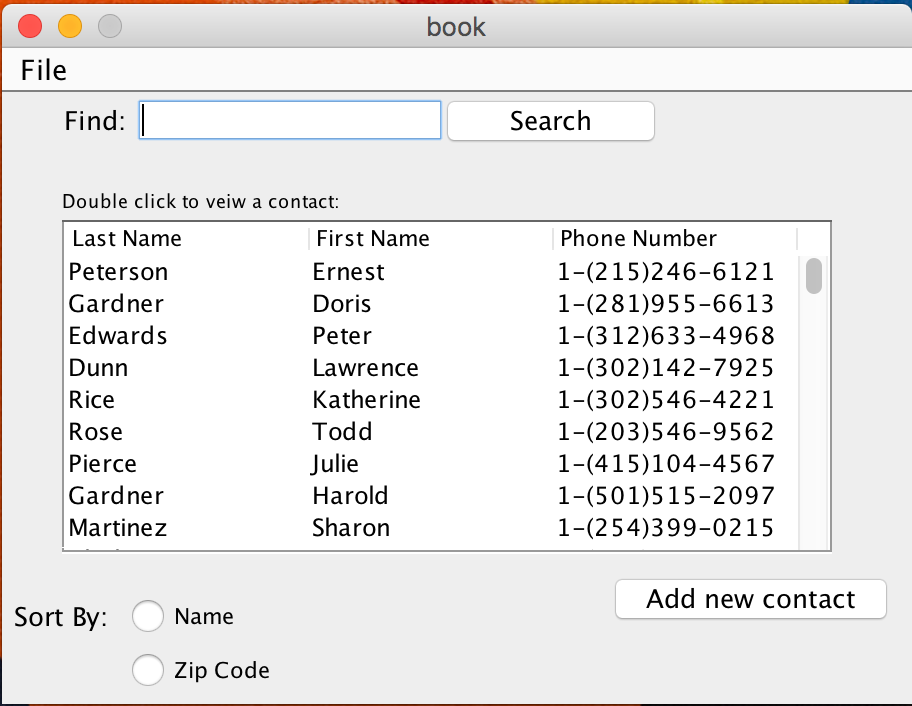
\includegraphics[width=250]{main_page_full.png}
      \caption{Full Main Page}
    \end{figure}
    
    \item{\textbf{Select the File Menu}}\\ At the top of the Main page window there will be a button that reads "File". Select it and a menu will pop open.
    
    \begin{figure}[h!]
    \centering
      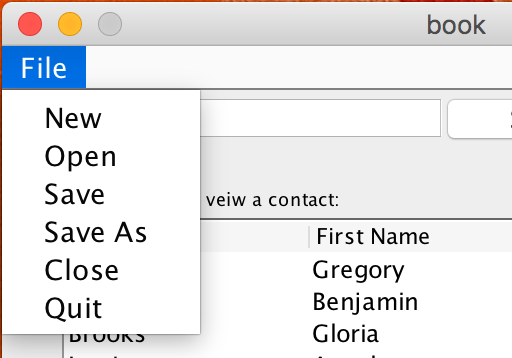
\includegraphics[width=250]{file_menu.png}
      \caption{File Menu}
    \end{figure}   
    
    \clearpage
    
    \item{\textbf{Select "Open"}}\\ Click the "Open" button and a pop up window will appear.
    
    \begin{figure}[h!]
    \centering
      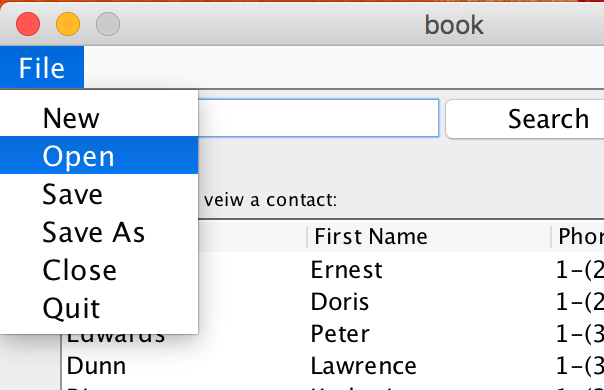
\includegraphics[width=250]{open_selection.png}
      \caption{Select Open}
    \end{figure}
    
    \item{\textbf{Select File}}\\ In the new window you will be shown a list of file names. Any file names that end in ".tsv" can be opened by the Address Book application. Select the file you wish to Open and then click the "Open" button. Upon clicking "Open" the Address Book you chose will appear.
    
    \begin{figure}[h!]
    \centering
      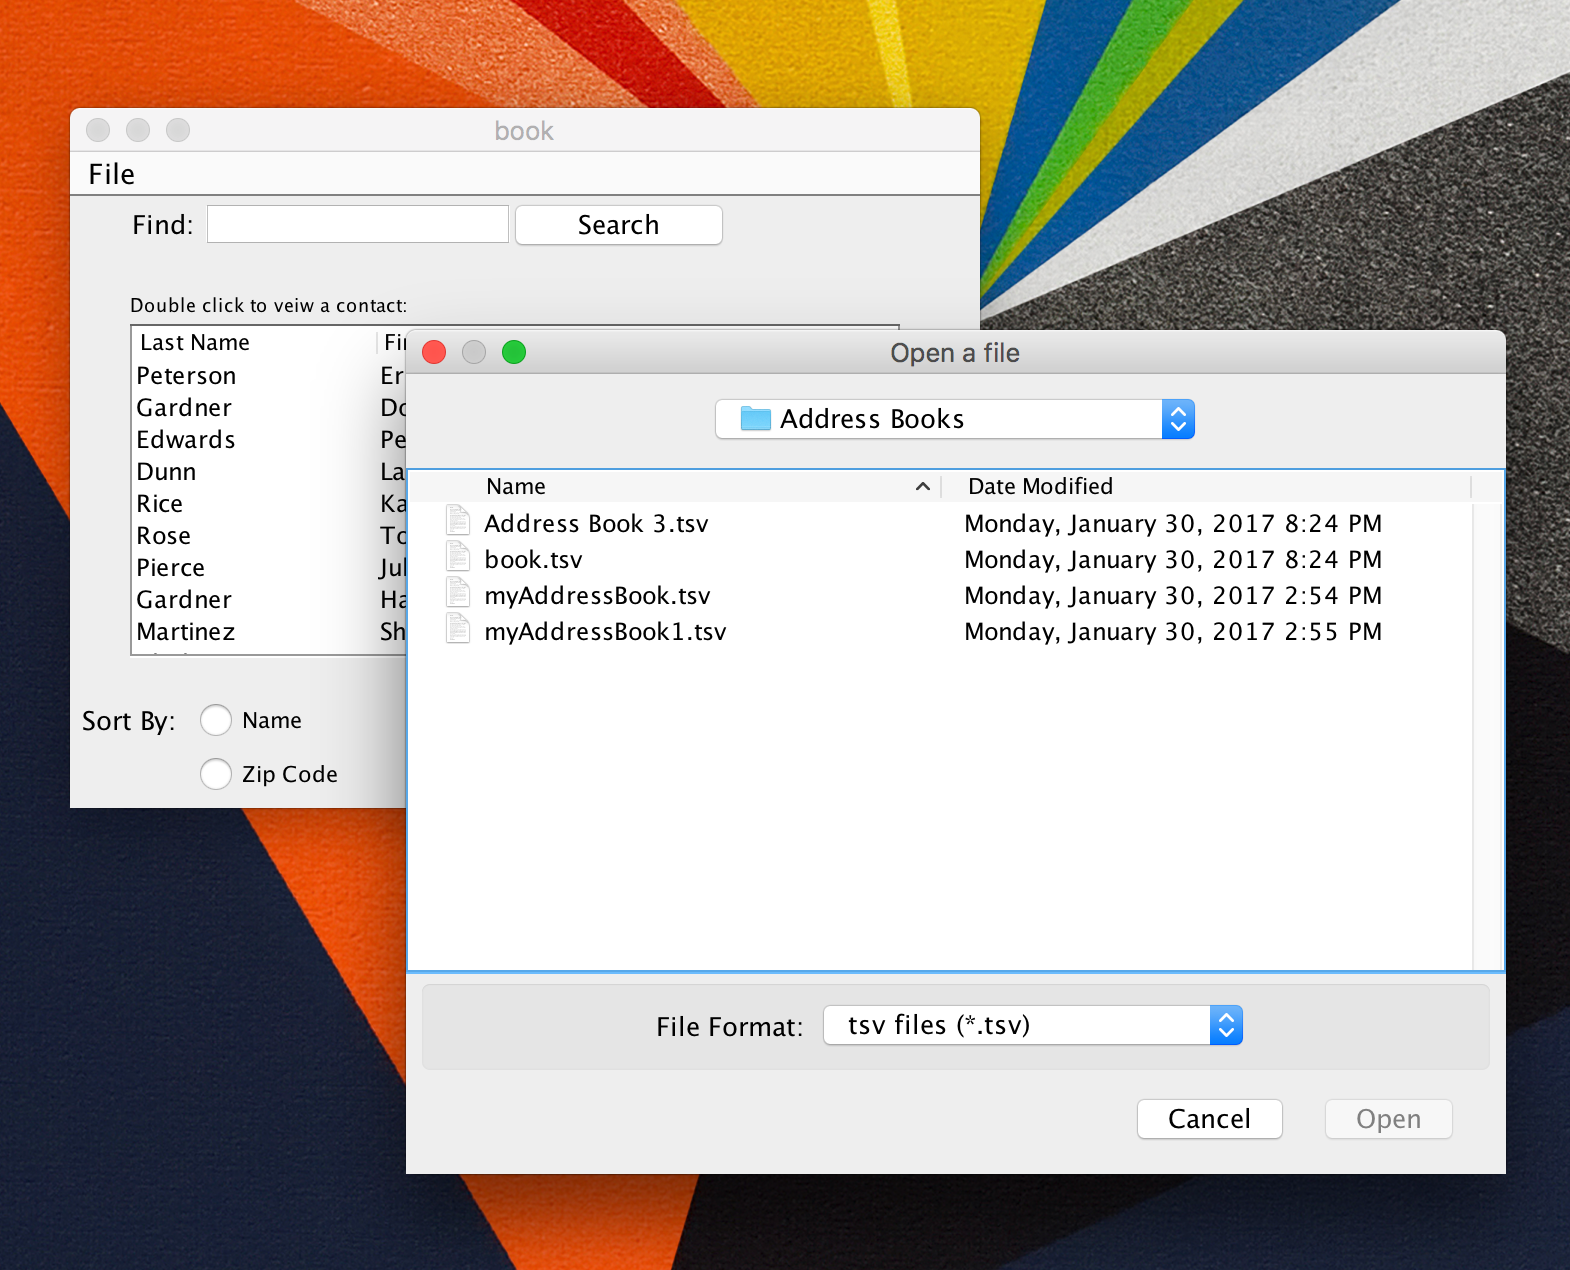
\includegraphics[width=250]{open_window.png}
      \caption{Open Window}
    \end{figure}
    
\end{enumerate}

\clearpage

\section{Close Address Book}
\subsection{Overview}
You can Close an Open Address Book by following the procedure below.
\subsection{Procedure}
\begin{enumerate}[label=\textbf{\arabic*})]
    \item{\textbf{Begin at the Main Page of the Address Book}}\\ Make sure you are at the Main page of the Address Book.
    
    \begin{figure}[h!]
    \centering
      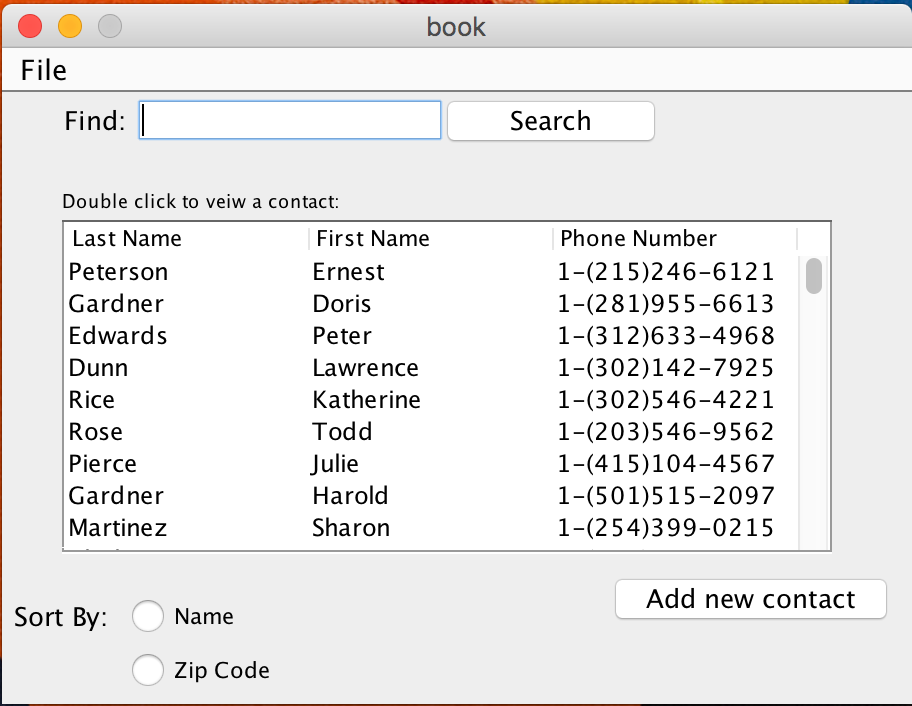
\includegraphics[width=250]{main_page_full.png}
      \caption{Full Main Page}
    \end{figure}
    
    \item{\textbf{Select the File Menu}}\\ At the top of the Main page window there will be a button that reads "File". Select it and a menu will pop open.
    
    \begin{figure}[h!]
    \centering
      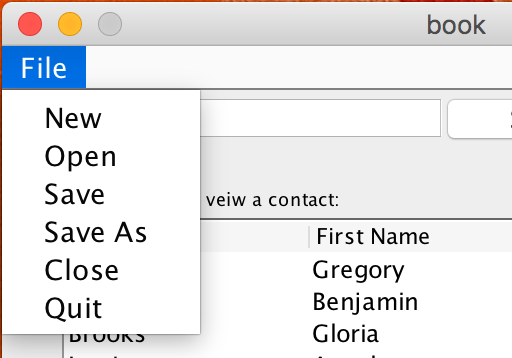
\includegraphics[width=250]{file_menu.png}
      \caption{File Menu}
    \end{figure}   
    
    \clearpage
    
    \item{\textbf{Select "Close"}}\\ Click the "Close" and the Address Book will close. Unless the Address Book has not been previously saved, then a pop up will appear prompting you to Save the file.
    
    \begin{figure}[h!]
    \centering
      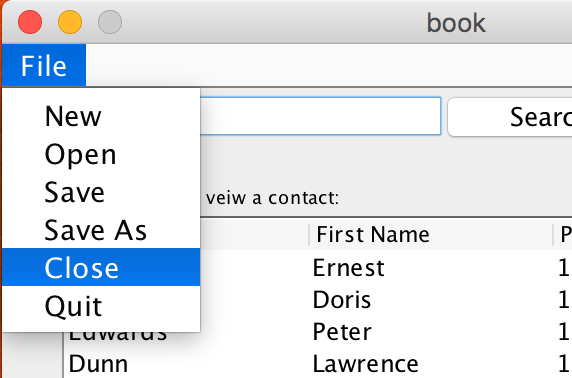
\includegraphics[width=250]{close_selection.png}
      \caption{Select Close}
    \end{figure}
    
    \begin{figure}[h!]
    \centering
      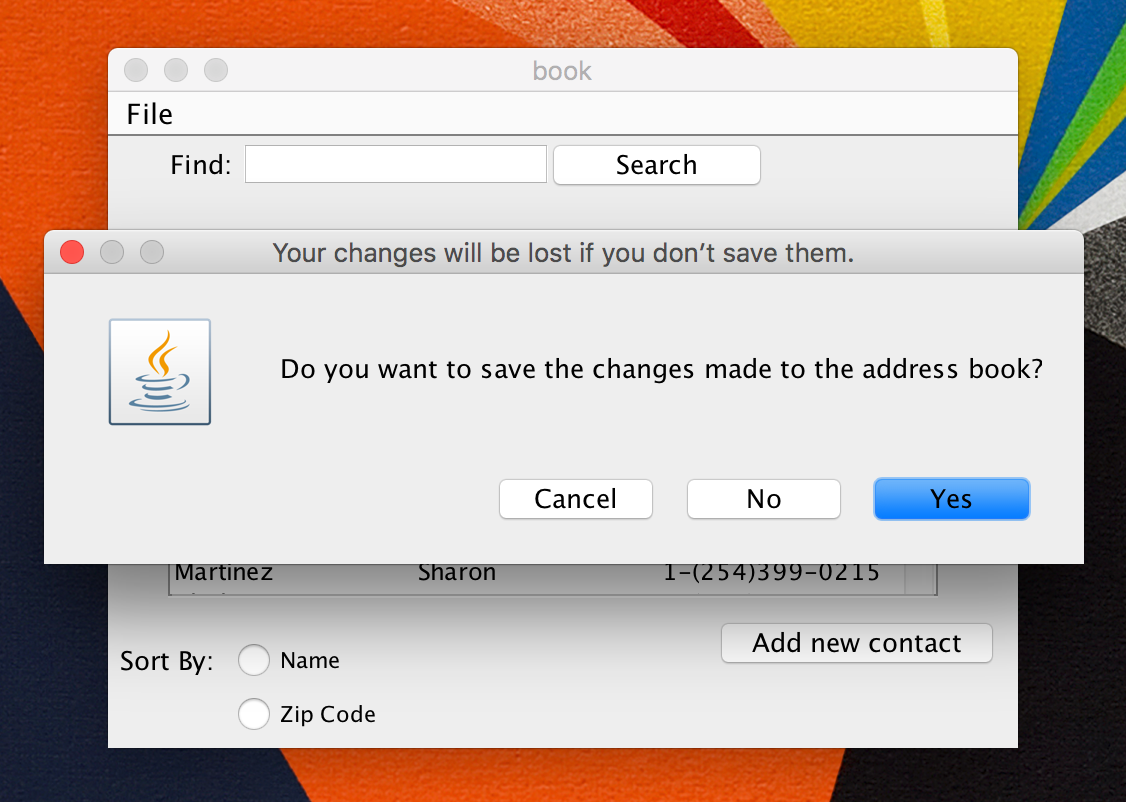
\includegraphics[width=250]{close_save_error.png}
      \caption{Save Prompt}
    \end{figure} 
\end{enumerate}

\clearpage

\section{Quitting the Application}
\subsection{Overview}
If you wish to stop using the Address Book application follow the procedure below to do so. 
\subsection{Procedure}
\begin{enumerate}[label=\textbf{\arabic*})]
    \item{\textbf{Begin at the Main Page of the Address Book}}\\ Make sure you are at the Main page of the Address Book.
    
    \begin{figure}[h!]
    \centering
      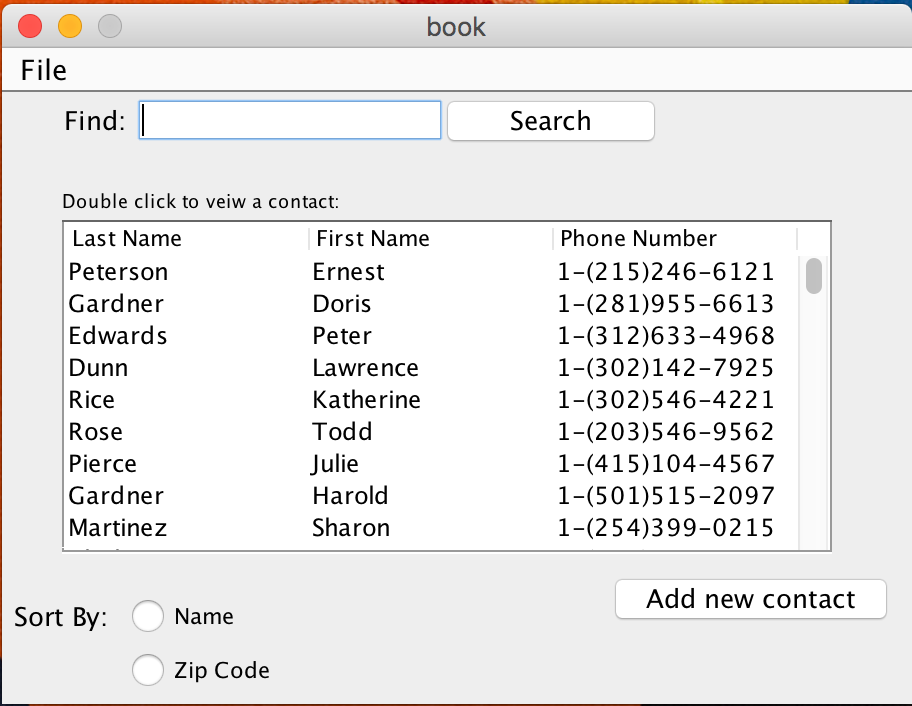
\includegraphics[width=250]{main_page_full.png}
      \caption{Full Main Page}
    \end{figure}
    
    \item{\textbf{Select the File Menu}}\\ At the top of the Main page window there will be a button that reads "File". Select it and a menu will pop open.
    
    \begin{figure}[h!]
    \centering
      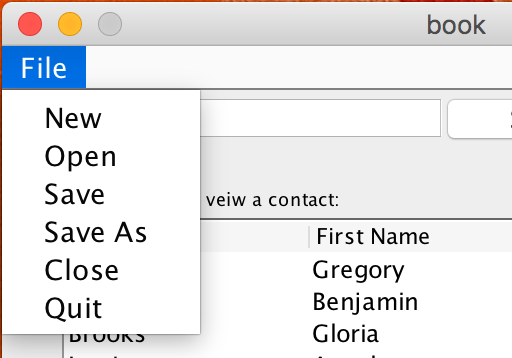
\includegraphics[width=250]{file_menu.png}
      \caption{File Menu}
    \end{figure} 
    
    \clearpage
    
    \item{\textbf{Select "Quit"}}\\ Click the "Quit" and the Address Book application will close. Unless the Address Book(s) haven't been previously saved, then a pop up will appear prompting you to Save the file(s).
    
    \begin{figure}[h!]
    \centering
      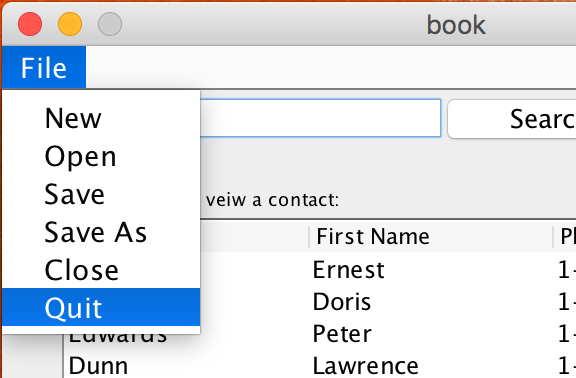
\includegraphics[width=250]{quit_selection.png}
      \caption{Select Quit}
    \end{figure}
    
    \begin{figure}[h!]
    \centering
      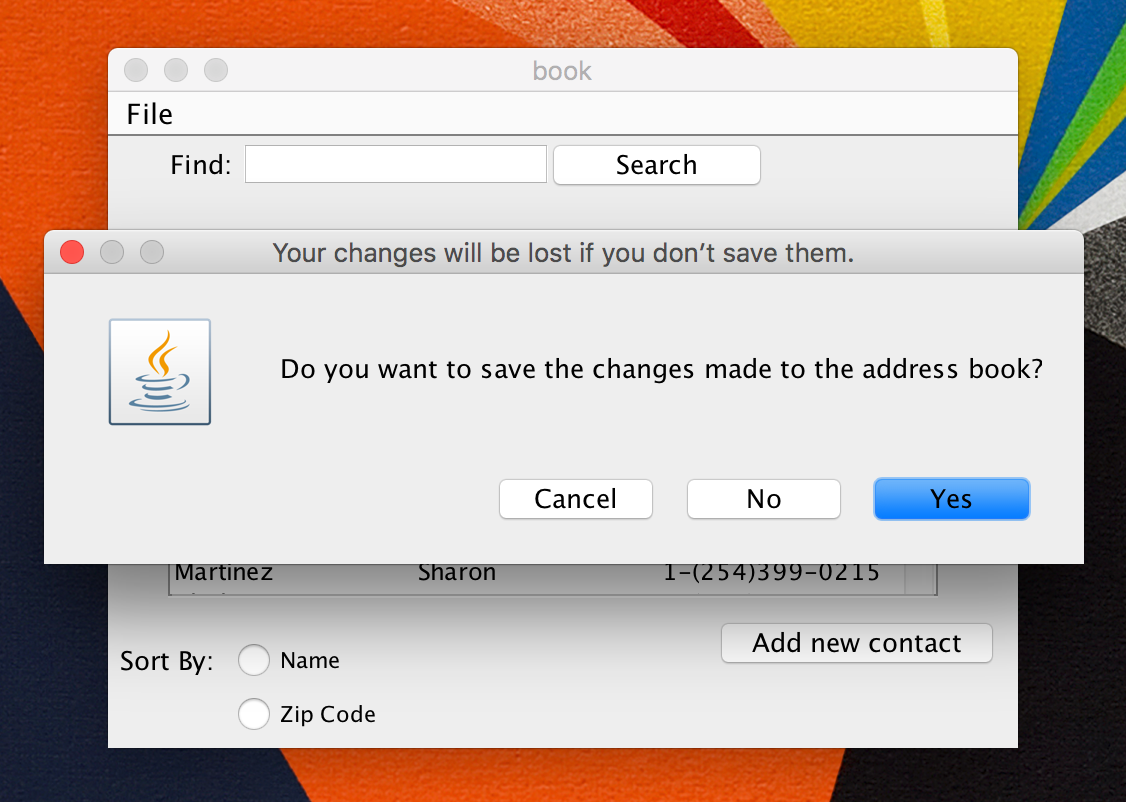
\includegraphics[width=250]{close_save_error.png}
      \caption{Save Prompt}
    \end{figure} 
\end{enumerate}

\clearpage

\end{document}